\documentclass[12pt,a4paper]{article}
\usepackage[margin=2.4cm]{geometry}
\usepackage[T1]{fontenc}
\usepackage[utf8]{inputenc}
\usepackage{graphicx}
\usepackage{xcolor}
\usepackage{listings}
\usepackage{hyperref}
\usepackage{titlesec}
\usepackage{fancyhdr}
\usepackage{setspace}
\usepackage{booktabs}

\definecolor{brand}{HTML}{006C47}
\hypersetup{colorlinks=true,linkcolor=brand,urlcolor=brand}
\titleformat{\section}{\Large\bfseries\color{brand}}{\thesection}{0.8em}{}
\pagestyle{fancy}
\setlength{\headheight}{14pt}
\fancyhf{}
\fancyhead[L]{\small Consumo del servicio de login}
\fancyhead[R]{\small Recurrly}
\fancyfoot[C]{\thepage}
\renewcommand{\headrulewidth}{0.4pt}

\lstset{
  basicstyle=\ttfamily\small,
  breaklines=true,
  frame=single,
  backgroundcolor=\color{black!4}
}

\begin{document}

\begin{titlepage}
\centering
\vspace*{1.6cm}
{\large Universidad de Oriente --- UNIVO\par}
\vspace{0.4cm}
{\large Desarrollo de aplicaciones m\'oviles\par}
\vspace{1.8cm}
{\color{brand}\rule{\textwidth}{1.2pt}\par}
\vspace{0.8cm}
{\Huge\bfseries Consumo del Servicio de Login\par}
\vspace{0.5cm}
{\Large Recurrly --- Expo / React Native\par}
\vspace{0.8cm}
{\color{brand}\rule{\textwidth}{1.2pt}\par}
\vspace{1.6cm}
\begin{tabular}{rl}
\textbf{Clase:} & 7 --- 10/08/2026\\
\textbf{Actividad:} & Consumo del servicio de login\\
\textbf{Patr\'on:} & MVVM\\
\textbf{Cliente HTTP:} & Axios\\
\textbf{API:} & \texttt{https://api-ecommerce-5aby.onrender.com}\\
\textbf{Endpoint:} & \texttt{POST /auth/login}\\
\textbf{Rama:} & \texttt{feat/consumo-servicio-login}\\
\end{tabular}
\vfill
{\large Androso\par}
{\large 6 de septiembre de 2026\par}
\end{titlepage}

\section{Objetivo}
Implementar el inicio de sesi\'on contra el API REST remoto usando Axios, organizar la soluci\'on con MVVM y comprobar en consola que el token de sesi\'on llega correctamente. Tambi\'en se documenta el caso de error del servidor.

La clase (Notion: \emph{Clase 7 --- Consumo del servicio de login}) pide exactamente esta separaci\'on: la vista no carga la l\'ogica; \texttt{useLogin} aísla estado, validaci\'on y llamada HTTP; \texttt{auth.service.ts} centraliza el consumo de \texttt{POST /auth/login}.

\section{Arquitectura MVVM}
\begin{tabular}{llp{8.2cm}}
\toprule
Capa & Archivo & Responsabilidad \\
\midrule
Model & \texttt{src/auth/models/auth.model.ts} & Interfaces \texttt{Role}, \texttt{UserResponse} y \texttt{AuthResponse} alineadas a la respuesta real del backend (\texttt{token} + \texttt{userResponse}). \\
Service & \texttt{src/auth/service/auth.service.ts} & \texttt{AuthService.login} con \texttt{axios.post} y mapeo de \texttt{error.response.data.message}. \\
ViewModel & \texttt{src/auth/viewmodels/use-login.ts} & Estado, validaci\'on, \texttt{isLoading}, impresi\'on del token y manejo de error. \\
View & \texttt{app/(public)/index.tsx} & Pantalla de login: campos, \texttt{AuthError} y \texttt{ActivityIndicator}. \\
\bottomrule
\end{tabular}

Los nombres del JSON real del API son \texttt{userResponse} y \texttt{lastName} (no \texttt{user}/\texttt{lastname} de las notas de clase). El modelo TypeScript sigue el contrato verificado en Postman/curl.

\section{Consumo del endpoint}
Base URL: \texttt{EXPO\_PUBLIC\_API\_URL} o, por defecto, \texttt{https://api-ecommerce-5aby.onrender.com}.

Cuerpo enviado:
\begin{lstlisting}
{ "email": string, "password": string }
\end{lstlisting}

Respuesta exitosa: HTTP 200 con JWT en \texttt{token} (prefijo \texttt{Bearer}) y datos de usuario en \texttt{userResponse}.

Error de credenciales: HTTP 401
\begin{lstlisting}
{"statusCode":401,"message":"El email o Password no son validos"}
\end{lstlisting}

En el ViewModel, tras un login correcto se ejecuta:
\begin{lstlisting}
console.log('[Auth] Session token received:', session.token);
\end{lstlisting}
y en fallo:
\begin{lstlisting}
console.error('[Auth] Login failed:', message);
\end{lstlisting}

\section{Caso de error del servidor}
Credenciales inv\'alidas. El API responde 401 y la vista muestra el mensaje del servidor.

\begin{figure}[h]
\centering
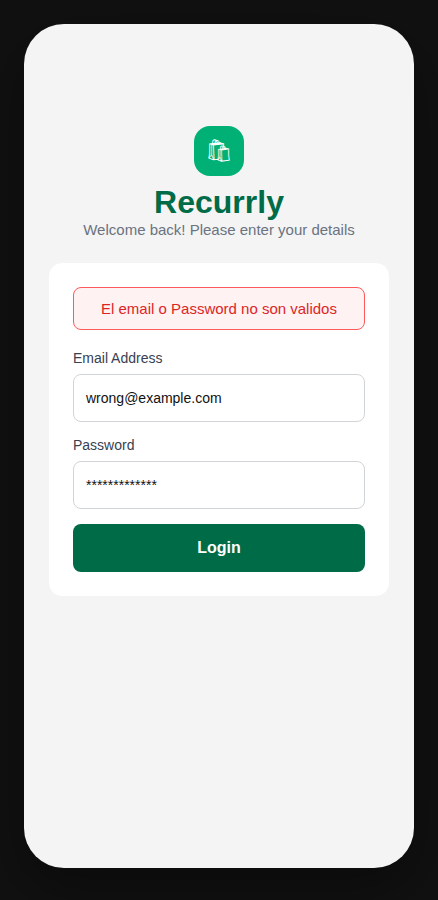
\includegraphics[width=0.42\textwidth]{assets/error-login.png}
\caption{Pantalla de login mostrando el error del API.}
\end{figure}

\begin{figure}[h]
\centering
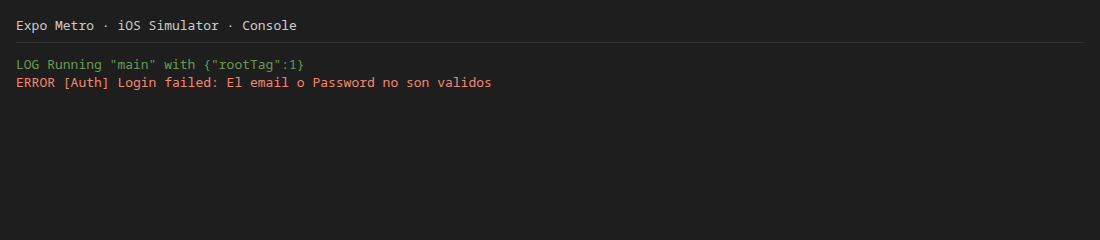
\includegraphics[width=0.95\textwidth]{assets/error-console.png}
\caption{Salida de depuraci\'on del error de login.}
\end{figure}

\section{Caso de \'exito: token de sesi\'on}
Login correcto con usuario de prueba. El token se imprime en la consola de Metro, tal como pide la clase (\texttt{handleLogin} imprime el token despu\'es de \texttt{AuthService.login()}).

\begin{figure}[h]
\centering
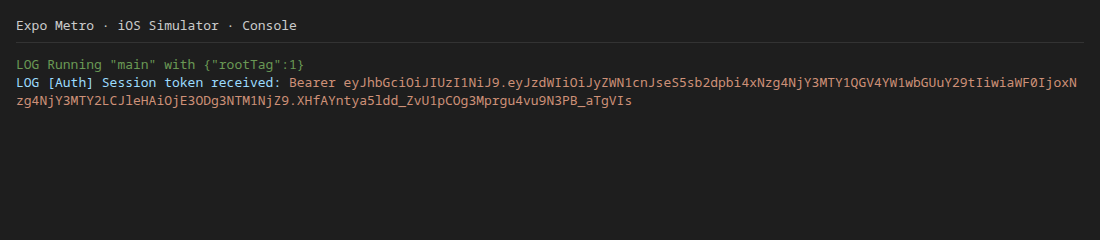
\includegraphics[width=0.95\textwidth]{assets/success-token.png}
\caption{Token de sesi\'on recibido e impreso en consola.}
\end{figure}

Usuario de verificaci\'on: \texttt{recurrly.login.1788667165@example.com} (id 352). El JWT llega con el prefijo \texttt{Bearer}.

\section{Conclusi\'on}
El servicio de login queda consumido con Axios, tipado, separado en MVVM y con evidencia de error 401 y de token en consola. La vista solo presenta; el hook orquesta; el servicio habla con Render.

\end{document}
